%%%%%%%%%%%%%%%%%%%%%%%%%%%%%%%%%%%%%%%%%%%%%%%%%%%%%%%%%%%%%%%%%%%%%%
% Lớp 11 | Hàm số lượng giác và phương trình lượng giác | Góc lượng giác
% Dạng 1D1?1-2: Chuyển đổi đơn vị độ và radian
% Số câu: 59  (sinh tự động bởi tach_cau.py; từ nay thầy sửa trực tiếp file này)
%%%%%%%%%%%%%%%%%%%%%%%%%%%%%%%%%%%%%%%%%%%%%%%%%%%%%%%%%%%%%%%%%%%%%%

%%%%%%%%%%%%%%%% TRẮC NGHIỆM 4 PHƯƠNG ÁN %%%%%%%%%%%%%%%%

% nguồn: Ok_Toan11_TracNghiem_Lan2
\begin{ex}%[1D1N1-2]%[ma:bdfdf082]
	Đổi số đo của góc $10\,\mathrm{rad}$ sang đơn vị độ, phút, giây,  ta được
	\choice 
		{\True $572^\circ  57'28''$}
		 {$1800^\circ$}
		 {$\dfrac{\pi}{18}$}
		{$527^\circ 57'28''$} 
	 \loigiai{
		Tính được $10\,\mathrm{rad}= \dfrac{10}{\pi} \cdot 180^\circ \approx  572^\circ 57'28''$.
	} 
\end{ex}

% nguồn: Ok_Toan11_TracNghiem_Lan2
\begin{ex}%[1D1N1-2]%[ma:ce64b2b5]
	Góc $70^\circ$ có số đo bằng rađian là 
	\choice 
		{$\dfrac{18\pi}{7}$} 
		{\True  $\dfrac{7\pi}{18}$}
		{$\dfrac{9\pi}{7}$} 
		 {$\dfrac{7\pi}{9}$}
	 \loigiai{
		Khi đổi góc  $70^\circ$ sang đơn vị rađian, ta có $70 \cdot \dfrac{\pi}{180} = \dfrac{7\pi}{18}$.
	} 
\end{ex}

% nguồn: Ok_Toan11_TracNghiem_Lan2
\begin{ex}%[1D1N1-2]%[ma:91f4c69a]
	 Góc có số đo $\dfrac{-7\pi}{4}$ thì góc đó có số đo là
	\choice 
		 {\True $-315^\circ$}
		 {$-630^\circ$}
		{$-1^\circ  45'$}
		 {$-135^\circ$}
	\loigiai{ 
		Góc có số đo $\dfrac{-7\pi}{4}$ tương đương với số đo $\dfrac{-7 \cdot 180^\circ}{4}  = -315^\circ$.
	} 
\end{ex}

% nguồn: Ok_Toan11_TracNghiem_Lan2
\begin{ex}%[1D1N1-2]%[ma:32aab219]
	Nếu  một cung tròn có số đo là $a^\circ$ thì số đo rađian của nó là
	\choice 
		{$180\pi  a$}
		{$\dfrac{180\pi}{a}$} 
		{\True $\dfrac{a\pi}{180}$} 
		 {$\dfrac{\pi}{180a}$}
	 \loigiai{
		Số đo  rađian của một cung tròn có số đo $a^\circ$ là $\dfrac{a\pi}{180}$.
	 }
\end{ex}

% nguồn: Ok_Toan11_TracNghiem_Lan2
\begin{ex}%[1D1N1-2]%[ma:5996c798]
	Góc có số đo $120^\circ$ đổi sang  rađian là
	 \choice
		 {$\dfrac{3\pi}{2}$}
		{\True $\dfrac{2\pi}{3}$} 
		{$\dfrac{\pi}{4}$} 
		{$\dfrac{\pi}{10}$} 
	\loigiai{ 
		Khi đổi góc $120^\circ$ sang đơn vị rađian, ta có $120 \cdot \dfrac{\pi}{180} = \dfrac{2\pi}{3}$. 
	} 
\end{ex}

% nguồn: Ok_Toan11_TracNghiem_Lan2
\begin{ex}%[1D1N1-2]%[ma:0b4d99dd]
	Góc có số đo $108^\circ$ đổi ra rađian là 
	\choice 
		{\True $\dfrac{3\pi}{5}$} 
		 {$\dfrac{\pi}{10}$}
		{$\dfrac{3\pi}{2}$} 
		 {$\dfrac{\pi}{4}$}
	 \loigiai{
		Ta có $108^\circ = \dfrac{108^{\circ} \cdot \pi}{180^{\circ}} =  \dfrac{3\pi}{5}$.
	 }
\end{ex}

% nguồn: Ok_Toan11_TracNghiem_Lan2
\begin{ex}%[1D1N1-2]%[ma:1d5ef6b2]
	Cho góc có số đo $405^\circ$, khi đổi góc này sang đơn vị rađian  ta được
	\choice 
		 {$\dfrac{8\pi}{9}$}
		 {\True $\dfrac{9\pi}{4}$}
		{$\dfrac{9}{4}$} 
		{$\dfrac{9\pi}{8}$} 
	 \loigiai{
		Khi  đổi góc $405^\circ$ sang đơn vị rađian, ta có $405 \cdot \dfrac{\pi}{180} = \dfrac{9\pi}{4}$.
	 }
\end{ex}

% nguồn: Ok_Toan11_TracNghiem_Lan2
\begin{ex}%[1D1N1-2]%[ma:947ecd94]
	Số  đo theo đơn vị rađian của góc $405^\circ$ là
	\choice 
		{\True $\dfrac{9\pi}{4}$} 
		{$\dfrac{7\pi}{4}$} 
		 {$\dfrac{5\pi}{4}$}
		 {$\dfrac{4\pi}{7}$}
	\loigiai{ 
		Khi đổi góc $405^\circ$  sang đơn vị rađian, ta có $405 \cdot \dfrac{\pi}{180} = \dfrac{9\pi}{4}$.
	 }
\end{ex}

% nguồn: Ok_TracNghiemLop11_Lan1
\begin{ex}%[1D1N1-2]%[ma:0261e045]
	Góc có số đo  $\dfrac{\pi}{9}$ đổi sang độ là
	 \choice
		 {$15^{\circ}$}
		 {$18^{\circ}$}
		{\True  $20^{\circ}$}
		 {$25^{\circ}$}
	\loigiai{ 
		Áp dụng công thức đổi  rad sang độ $n=\dfrac{\alpha \cdot 180}{\pi}$.
		Ta có $n=\dfrac{\pi}{9} \cdot  \dfrac{180^{\circ}}{\pi}=20^{\circ}.
		$ 
	 }
\end{ex}

% nguồn: Ok_TracNghiemLop11_Lan1
\begin{ex}%[1D1N1-2]%[ma:1c21620b]
	Khi đổi $\dfrac{5\pi }{3}\,\mathrm{rad}$ sang đơn vị  độ ta được kết quả là
	\choice 
		{$360^\circ$} 
		{\True  $300^\circ$}
		{$250^\circ$} 
		{$270^\circ$} 
	 \loigiai{
		Ta có  $\dfrac{5\pi }{3}\,\mathrm{rad}=\left(\dfrac{5\pi }{3}\,\cdot \dfrac{180}{\pi }\right)^\circ=300^\circ$.
	 }
\end{ex}

% nguồn: Ok_TracNghiemLop11_Lan1
\begin{ex}%[1D1N1-2]%[ma:651d5e34]
	Góc $-120^\circ$ có số đo  bằng radian là
	\choice 
		{$-\dfrac{5\pi}{6}$} 
		 {$-\dfrac{\pi}{6}$}
		 {\True $-\dfrac{2\pi}{3}$}
		{$-\dfrac{\pi}{3}$} 
	\loigiai{ 
		 Ta có $-120^\circ=-120^\circ\cdot\dfrac{\pi}{180^\circ}=-\dfrac{2\pi}{3}$.
	} 
\end{ex}

% nguồn: Ok_TracNghiemLop11_Lan1
\begin{ex}%[1D1N1-2]%[ma:ab73dfd2]
	Nếu một góc có số đo $\dfrac{5\pi}{12}$ rad thì số đo  của góc đó khi đổi sang đơn vị độ, phút, giây là
	\choice 
		 {$45^\circ$}
		 {\True $75^\circ$}
		{$55^\circ$} 
		{$65^\circ$} 
	\loigiai{ 
		Ta có $1$ rad $=\left(\dfrac{180}{\pi} \right)^\circ \Rightarrow \dfrac{5\pi}{12}$  rad $=\left(\dfrac{180}{\pi}\cdot \dfrac{5\pi}{12} \right)^\circ=75^\circ$.
	} 
\end{ex}

% nguồn: Ok_TracNghiemLop11_Lan1
\begin{ex}%[1D1N1-2]%[ma:b1a4ee27]
	Số đo radian của  góc $135^\circ$ là
	\choice 
		 {$\dfrac{\pi}{6}$}
		 {\True $\dfrac{3\pi}{4}$}
		{$\dfrac{2\pi}{3}$} 
		 {$\dfrac{\pi}{2}$}
	 \loigiai{
		Sử dụng máy tính bỏ túi ta  tính được $135^\circ=\dfrac{3\pi}{4}$.
	} 
\end{ex}

% nguồn: Ok_TracNghiemLop11_Lan1
\begin{ex}%[1D1N1-2]%[ma:44a64662]
	Góc có số  đo $130^\circ$ đổi sang rađian là
	\choice 
		{\True $\dfrac{13\pi}{18}$} 
		{$\dfrac{13}{18}$} 
		 {$\dfrac{18\pi}{13}$}
		 {$\dfrac{18}{13}$}
	 \loigiai{
		Áp dụng công thức $\alpha^\circ=\dfrac{\alpha \pi}{180} rad$  ta được $130^\circ=\dfrac{13\pi}{18}$.
	 }
\end{ex}

% nguồn: Ok_TracNghiemLop11_Lan1
\begin{ex}%[1D1N1-2]%[ma:f623420a]
	Góc có số đo $-\dfrac{3\pi}{16}$ có số đo theo độ  là
	 \choice
		 {$33^{\circ} 45'$}
		{$-29^{\circ} 30'$} 
		{$-32^{\circ}  55'$}
		{\True $-33^{\circ} 45'$} 
	 \loigiai{
		Vì $1$ rad  $=\left(\dfrac{180}{\pi} \right)^{\circ}$ nên $\dfrac{-3\pi}{16}=\left(\dfrac{-3\pi}{16} \cdot \dfrac{180}{\pi} \right)^{\circ}=\left(\dfrac{-135}{4} \right)^{\circ}=-33,75^{\circ}=-33^{\circ} 45'$.
	 }
\end{ex}

% nguồn: Ok_TracNghiemLop11_Lan1
\begin{ex}%[1D1N1-2]%[ma:43f73d0a]
	 Nếu một cung tròn có số đo là $20$ độ thì số đo radian của nó là
	 \choice
		{$\dfrac{\pi}{10}$} 
		{\True  $\dfrac{\pi}{9}$}
		{$\dfrac{\pi}{8}$} 
		{$\dfrac{\pi}{11}$} 
	 \loigiai{
		Sử dụng công thức:  $\alpha^\circ=\alpha \cdot \dfrac{\pi}{180} \mathrm{rad}$. Ta có: $20^\circ=20 \cdot \dfrac{\pi}{180}=\dfrac{\pi}{9}$.
	 }
\end{ex}

% nguồn: Ok_TracNghiemLop11_Lan1
\begin{ex}%[1D1N1-2]%[ma:b6e18f34]
	Giả sử các đẳng  thức đều có nghĩa. Chọn khẳng định đúng trong các khẳng định sau.
	 \choice
		{$\sin^2  \alpha+\cos^2\alpha=-1$}
		{\True $\tan \alpha \cdot  \cot \alpha=1$}
		{$1+\tan^2 \alpha=\dfrac{1}{\sin^2\alpha}$} 
		 {$1+\cot^2 \alpha=\dfrac{1}{\cos^2\alpha}$}
	 \loigiai{Theo tính chất ta có
		\begin{enumerate}
			 \item $\sin^2 \alpha+\cos^2\alpha=1$.
			\item $\tan \alpha \cdot \cot \alpha=1$. 
			\item $1+\tan^2  \alpha=\dfrac{1}{\cos^2\alpha}$.
			 \item $1+\cot^2 \alpha=\dfrac{1}{\sin^2\alpha}$.
		\end{enumerate}
	} 
\end{ex}

% nguồn: Ok_TracNghiemLop11_Lan1
\begin{ex}%[1D1N1-2]%[ma:2d1c8986]
	Cho góc $\alpha \in  \left(\dfrac{\pi}{2};\pi\right)$. Chọn khẳng định đúng.
	\choice 
		 {\True $\cos \alpha <0 $}
		{$\sin \alpha <0 $} 
		{$\tan \alpha  >0 $}
		{$\cot \alpha >0  $}
	\loigiai{Giả sử điểm $M$ biểu diễn góc $\alpha \in  \left(\dfrac{\pi}{2};\pi\right)$.\\ Khi đó điểm $M$ thuộc cung phần tư thứ hai.\\
		Suy ra $\sin \alpha=y_M>0$; $\cos \alpha=x_M<0$; $\tan  \alpha=\dfrac{y_M}{x_M}<0 $; $\cot \alpha=\dfrac{x_M}{y_M}<0$.
	} 
\end{ex}

% nguồn: Ok_TracNghiemLop11_Lan1
\begin{ex}%[1D1N1-2]%[ma:68e7c5f5]
	Cho  góc có số đo $108^\circ$ đổi ra rađian là
	\choice 
		 {$\dfrac{\pi}{10}$}
		 {$\dfrac{3\pi}{2}$}
		{$\dfrac{\pi}{4}$} 
		{\True  $\dfrac{3\pi}{5}$}
	 \loigiai{
	Ta có $108^\circ=\dfrac{108^\circ\cdot\pi}{180^\circ} =\dfrac{3\pi}{5}$.} 
\end{ex}

% nguồn: Ok_TracNghiemLop11_Lan1
\begin{ex}%[1D1N1-2]%[ma:455b3202]
	Đổi số đo góc  $105^{\circ}$ sang rađian bằng
	 \choice
		{$\dfrac{5\pi}{12}$} 
		{\True  $\dfrac{7\pi}{12}$}
		{$\dfrac{9\pi}{12}$} 
		 {$\dfrac{5\pi}{8}$}
	 \loigiai{
		\[105^{\circ}=\dfrac{105^{\circ}\cdot  \pi}{180^{\circ}}=\dfrac{7\pi}{12}.
		\] 
	} 
\end{ex}

% nguồn: Ok_TracNghiemLop11_Lan1
\begin{ex}%[1D1N1-2]%[ma:33bceab1]
	Đổi sang radian góc có số đo $108^\circ$ ta được 
	 \choice
		{$\dfrac{\pi}{4}$} 
		{$\dfrac{\pi}{10}$} 
		 {$\dfrac{3\pi}{2}$}
		 {\True $\dfrac{3\pi}{5}$}
	 \loigiai{
		Ta có $1^\circ=\dfrac{\pi}{180}$  nên $108^\circ=\dfrac{108\pi}{180}$ $=\dfrac{3\pi}{5}$.
	 }
\end{ex}

% nguồn: Ok_TracNghiemLop11_Lan1
\begin{ex}%[1D1N1-2]%[ma:61d14748]
	Cho góc lượng giác $(OA,OB)$ có số đo bằng $\dfrac{\pi}{6}$. Hỏi  trong các số đo góc sau, số đo nào là số đo của một góc lượng giác có cùng tia đầu, tia cuối với góc lượng giác $(OA,OB)$?
	 \choice
		 {$\dfrac{-49\pi}{6}$}
		{$-\dfrac{7\pi}{6}$} 
		{$\dfrac{7\pi}{6}$} 
		 {\True $\dfrac{49\pi}{6}$}
	\loigiai{ 
		Áp dụng kiến thức: Số đo của các góc lượng giác có chung tia đầu, tia cuối sai khác nhau một bội nguyên của $2\pi$.\\ 
	Ta thấy $\dfrac{49\pi}{6}-\dfrac{\pi}{6}=4\cdot2\pi$.} 
\end{ex}

% nguồn: Ok_TracNghiemLop11_Lan1
\begin{ex}%[1D1N1-2]%[ma:6a159087]
	Góc có số đo $45^{\circ}$ bằng bao  nhiêu radian
	 \choice
		{\True $\dfrac{\pi}{4}$} 
		 {$\dfrac{2\pi}{3}$}
		 {$\dfrac{\pi}{3}$}
		 {$\dfrac{\pi}{2}$}
	\loigiai{ 
		Ta có  $45^{\circ} = \dfrac{45 \cdot \pi}{180} = \dfrac{\pi}{4}$ rad.
	 }
\end{ex}

% nguồn: Ok_TracNghiemLop11_Lan1
\begin{ex}%[1D1B1-2]%[ma:f9062a7f]
	Hàm số $y=\sin  x$
	 \choice
		{đồng biến trên mỗi khoảng $\left(\dfrac{\pi}{2}+k2\pi;\pi+k2\pi\right)$ và nghịch biến trên mỗi khoảng  $\left(\pi+k2\pi;k2\pi\right)$ với $k\in\mathbb{Z}$}
		{đồng biến trên mỗi khoảng  $\left(-\dfrac{3\pi}{2}+k2\pi;\dfrac{5\pi}{2}+k2\pi\right)$ và nghịch biến trên mỗi khoảng $\left(-\dfrac{\pi}{2}+k2\pi;\dfrac{\pi}{2}+k2\pi\right)$ với $k\in\mathbb{Z}$}
		 {đồng biến trên mỗi khoảng $\left(\dfrac{\pi}{2}+k2\pi;\dfrac{3\pi}{2}+k2\pi\right)$ và nghịch biến trên mỗi khoảng $\left(-\dfrac{\pi}{2}+k2\pi;\dfrac{\pi}{2}+k2\pi\right)$ với $k\in\mathbb{Z}$}
		{\True đồng biến trên mỗi khoảng $\left(-\dfrac{\pi}{2}+k2\pi;\dfrac{\pi}{2}+k2\pi\right)$ và nghịch  biến trên mỗi khoảng $\left(\dfrac{\pi}{2}+k2\pi;\dfrac{3\pi}{2}+k2\pi\right)$ với $k\in\mathbb{Z}$}
	\loigiai{ 
	\immini{ 
		Hàm  số $y=\sin x$ đồng biến trên mỗi khoảng $\left(-\dfrac{\pi}{2}+k2\pi;\dfrac{\pi}{2}+k2\pi\right)$ và nghịch biến trên mỗi khoảng $\left(\dfrac{\pi}{2}+k2\pi;\dfrac{3\pi}{2}+k2\pi\right)$ với $k\in\mathbb{Z}$.}{
		\begin{tikzpicture}[scale=.7,font=\footnotesize,line join=round,line cap=round,>=stealth]
				\def\r{3}  \def\m{3.5}
				\def\f  (#1){(#1)}
				\draw[->] (-\r,0)--(\r+0.5,0) node[below] {$x$}node[above]  {$\cos x$};
				\draw[->] (0,-\r)--(0,\r+0.5) node[below  right] {$y$} node[left]{$\sin x$};
				\draw (0,0)  node [below left] {$O$};
				\foreach \x/\g/\z in {2.5/-45/1,-2.5/-135/-1}\fill[black] (\x,0) circle  (1pt)+(\g:0.4) node{$\z$};
				\foreach  \y/\g/\z in {2.5/135/1,-2.5/-135/-1}\fill[black] (0,\y) circle (1pt)+(\g:0.4) node{$\z$};
				\draw[color=white]  (0,0) circle (\r);
				\draw[-latex] (10:\r)  arc (10:70:\r);
				\draw (2.2,-0.2)  node{$2\pi$}
					(2.3,0.2)  node{$0$}
					(.2,2.1) node{$\tfrac{\pi}{2}$} 
					 (-.2,-2.1) node{$\tfrac{3\pi}{2}$}
					(-2.3,0.2) node{$\pi$}; 
				 \draw[-latex] (-10:\r) arc (-10:-70:\r);
				\draw (0,0)  circle (2.5);
				\draw  (2,3) circle (6pt) node{$+$}
					 (2,-3) circle (6pt) node{$-$};
			\end{tikzpicture}
	}} 
\end{ex}

% nguồn: Ok_TracNghiemLop11_Lan1
\begin{ex}%[1D1B1-2]%[ma:bc4cd830]
	Hàm số $y=\sin x$ đồng biến trong  khoảng nào sau đây?
	 \choice
		 {$\left(7\pi; \dfrac{15\pi}{2}\right)$}
		{$\left(-\dfrac{7\pi}{2}; -3\pi\right)$} 
		{\True  $\left(\dfrac{19\pi}{2}; 10\pi\right)$}
		{$\left(-6\pi; -5\pi \right)$} 
	\loigiai{ Hàm số $y=\sin x$ đồng biến trên từng khoảng $\left(-\dfrac{\pi}{2}+k2\pi; \dfrac{\pi}{2}+k2\pi \right), k\in \mathbb{Z}$.\\ Dễ thấy với $k=5$ thì $\left(\dfrac{19\pi}{2};  10\pi\right)\subset \left(-\dfrac{\pi}{2}+5\cdot 2\pi; \dfrac{\pi}{2}+5\cdot 2\pi \right)$. Vậy $y=\sin x$ đồng biến trong khoảng $\left(\dfrac{19\pi}{2}; 10\pi\right)$. }
\end{ex}

% nguồn: Ok_TracNghiemLop11_Lan1
\begin{ex}[c]%[1D1B1-2]%[ma:b9cf1ffb]
	 Với $x\in \left(\dfrac{31\pi}{4};\dfrac{33\pi}{4}\right)$, mệnh đề nào sau đây là đúng?
	\choice 
		{Hàm số $y=\cot x$  nghịch biến}
		{\True Hàm số  $y=\sin x$ đồng biến}
		{Hàm số $y=\cos x$ nghịch  biến}
		{Hàm số $y=\tan  x$ nghịch biến}
	\loigiai{ 
	Ta có $\left(\dfrac{31\pi}{4};\dfrac{33\pi}{4}\right)=\left(-\dfrac{\pi}{4}+8\pi;\dfrac{\pi}{4}+8\pi \right)$ thuộc góc phần tư thứ  I và II.}
\end{ex}

% nguồn: Ok_TracNghiemLop11_Lan1
\begin{ex}%[1D1B1-2]%[ma:481837d4]
	Hãy chọn khẳng định \textbf{sai} trong các khẳng định dưới đây: Trong  khoảng $\left(\dfrac{\pi}{2};\pi\right)$ thì
	\choice 
		{\True hàm số $y=\cot x$ là hàm số đồng biến} 
		{hàm số $y=\tan x$ là hàm số  đồng biến}
		{hàm số $y=\cos x$ là hàm  số nghịch biến}
		{hàm số  $y=\sin x$ là hàm số nghịch biến}
	\loigiai{ 
		Trong khoảng $\left(\dfrac{\pi}{2};\pi\right)$ thì hàm số  $y=\cot x$ là hàm số nghịch biến.
	 }
\end{ex}

% nguồn: Ok_TracNghiemLop11_Lan1
\begin{ex}%[1D1B1-2]%[ma:4807c63e]
	Hàm số $y=\tan  x$ đồng biến trên khoảng nào sau đây?
	\choice{\True  $\left(0;\dfrac{\pi}{2}\right)$}{$(0;\pi)$}{$\left(\dfrac{\pi}{2};2 \pi\right)$}{$\left(\dfrac{\pi}{2};\dfrac{5 \pi}{2}\right)$}
	\loigiai{ 
		Hàm số $y=\tan x$ luôn đồng biến trên các khoảng xác định, vậy nó  đồng biến trên khoảng $\left(0;\dfrac{\pi}{2}\right)$.
	} 
\end{ex}

% nguồn: Ok_TracNghiemLop11_Lan1
\begin{ex}%[1D1B1-2]%[ma:0468c355]
	Hàm số $y=\sqrt{3}+2\cos  x$ tăng trên khoảng
	\choice 
		 {$\left(-\dfrac{\pi}{6};\dfrac{\pi}{2}\right)$}
		{$\left(\dfrac{\pi}{2};\dfrac{3\pi}{2}\right)$} 
		{\True  $\left(\dfrac{7\pi}{6};2\pi\right)$}
		{$\left(\dfrac{\pi}{6};\dfrac{\pi}{2}\right)$} 
	\loigiai{ 
	\immini{ 
		Vì hàm số $y=\cos x$ đồng biến trên mỗi khoảng $\left(-\pi+k2\pi;k2\pi\right)$, $k\in\mathbb{Z}$ nên hàm số $y=\sqrt{3}+2\cos x$ cũng đồng biến trên  mỗi khoảng $\left(-\pi+k2\pi;k2\pi\right)$, $k\in\mathbb{Z}$.\\
		Vì  $\left(\dfrac{7\pi}{6};2\pi\right)\subset(\pi;2\pi)$ (với $k=1$) nên hàm số đồng biến trên khoảng $\left(\dfrac{7\pi}{6};2\pi\right)$.}
		{ 
		\begin{tikzpicture}[scale=.7,font=\footnotesize,line join=round,line cap=round,>=stealth]
				\def\r{3} \def\m{3.5} 
				\def\f (#1){(#1)} 
				\draw[->] (-\r,0)--(\r+0.5,0)  node[below] {$x$}node[above] {$\cos x$};
				\draw[->] (0,-\r)--(0,\r+0.5)  node[below right] {$y$} node[left]{$\sin x$};
				\draw (0,0)  node [below left] {$O$};
				 \foreach \x/\g/\z in {2.5/-45/1,-2.5/-135/-1}\fill[black] (\x,0) circle (1pt)+(\g:0.4) node{$\z$};
				\foreach \y/\g/\z in {2.5/135/1,-2.5/-135/-1}\fill[black] (0,\y) circle (1pt)+(\g:0.4) node{$\z$}; 
				\draw[color=white] (0,0)  circle (\r);
				\draw[-latex] (10:\r) arc  (10:70:\r);
				\draw (2.2,-0.2) node{$2\pi$} 
					(2.3,0.2) node{$0$} 
					 (.2,2.1) node{$\tfrac{\pi}{2}$}
					(-.2,-2.1)  node{$\tfrac{3\pi}{2}$}
					 (-2.3,0.2) node{$\pi$};
				\draw[-latex] (-10:\r)  arc (-10:-70:\r);
				\draw (0,0)  circle (2.5);
				\draw (2,3) circle  (6pt) node{$+$}
					(2,-3) circle (6pt) node{$-$}; 
			\end{tikzpicture}
		} 
	 }
\end{ex}

% nguồn: Ok_TracNghiemLop11_Lan1
\begin{ex}%[1D1B1-2]%[ma:ab81c995]
	Hàm số $ y=\sin x $ nghịch  biến trên khoảng nào dưới đây?
	\choice 
		{$ \left(\dfrac{5\pi}{4};\dfrac{7\pi}{4}\right) $} 
		{$ \True \left(\dfrac{3\pi}{4};\dfrac{5\pi}{4}\right)  $}
		{$  \left(\dfrac{3\pi}{2};\dfrac{7\pi}{4}\right) $}
		 {$ \left(\dfrac{7\pi}{4};\dfrac{9\pi}{4}\right) $}
	 \loigiai{
	Vì hàm số $ y=\sin x $ nghịch biến trên mỗi khoảng $ \left(\dfrac{\pi}{2}+k2\pi;\dfrac{3\pi}{2}+k2\pi\right) $ với $k \in \mathbb {Z}$ nên nhận thấy $  \left(\dfrac{3\pi}{4};\dfrac{5\pi}{4}\right) \subset \left(\dfrac{\pi}{2};\dfrac{3\pi}{2}\right) $, vậy trong khoảng này hàm số $ y=\sin x $ nghịch biến.}
\end{ex}

% nguồn: Ok_TracNghiemLop11_Lan1
\begin{ex}%[1D1B1-2]%[ma:cc4103ef]
	Hàm số $y= \cot x$ nghịch biến trên  khoảng nào sau đây?
	 \choice{$(0;2\pi)$}{$\left(\dfrac{\pi}{2};2 \pi\right)$}{\True $(-\pi;0)$}{$\left(\dfrac{\pi}{2};\dfrac{3 \pi}{2}\right)$}
	\loigiai{ 
		 Hàm số $y=\cot x$ luôn nghịch biến trên các khoảng xác định.\\
		Vậy hàm  số nghịch biến trên khoảng $(0;\pi)$.
	} 
\end{ex}

% nguồn: Ok_TracNghiemLop11_Lan1
\begin{ex}[c]%[1D1B1-2]%[ma:5f4257f5]
	Xét sự biến thiên của hàm số $ y=\cot  2x $. Trong các kết luận sau, kết luận nào \textbf{đúng}?
	\choice 
		{Hàm số đã cho đồng biến trên  khoảng $ \left(0;\dfrac{\pi}{4}\right) $ và $ \left(\dfrac{\pi}{3};\dfrac{\pi}{2}\right) $}
		 {Hàm số đã cho nghịch biến trên khoảng $ \left(0;\dfrac{\pi}{2}\right) $ và đồng biến trên khoảng $ \left(\dfrac{\pi}{2};\pi \right) $}
		{\True Hàm số đã cho nghịch biến trên  khoảng $ \left(\dfrac{\pi}{2};\pi\right) $}
		{Hàm  số đã cho nghịch biến trên khoảng $ \left(\dfrac{\pi}{2};\dfrac{3\pi}{2}\right) $}
	 \loigiai{
		Hàm số $ y=\cot x $ nghịch biến trên mỗi khoảng $ \left(k\pi;\pi+k\pi\right)$ với $ k\in \mathbb {Z} $.\\Suy ra hàm số $ y=\cot2x $ nghịch  biến khi
		\begin{eqnarray*}
			&  &k\pi<2x<\pi+k\pi\\
			 &\Leftrightarrow & \dfrac{k\pi}{2}<x<\dfrac{\pi}{2}+\dfrac{k\pi}{2}.
		\end{eqnarray*}
	Vậy hàm số $ y=\cot2x $ nghịch biến trên mỗi khoảng $ \left(\dfrac{k\pi}{2};\dfrac{\pi}{2}+\dfrac{k\pi}{2}\right),k\in \mathbb {Z}  $.}
\end{ex}

% nguồn: Ok_TracNghiemLop11_Lan1
\begin{ex}%[1D1B1-2]%[ma:604b6cec]
	Xét các mệnh đề sau:\\ 
	(I): $\forall x\in\left(\pi;\dfrac{3\pi}{2}\right)$ hàm  số $y=\dfrac{1}{\sin x}$ nghịch biến.\\
	(II):  $\forall x\in\left(\pi;\dfrac{3\pi}{2}\right)$ hàm số $y=\dfrac{1}{\cos x}$ nghịch biến.\\
	Hãy chọn mệnh đề đúng  trong các mệnh đề trên.
	\choice 
		 {Cả hai đúng}
		{Chỉ  (I) đúng}
		{\True  Chỉ (II) đúng}
		 {Cả hai sai}
	 \loigiai{
		Hàm số $y=\sin x$ nghịch biến trên $\left(\pi;\dfrac{3\pi}{2}\right)$ nên hàm  số $y=\dfrac{1}{\sin x}$ đồng biến trên $\left(\pi;\dfrac{3\pi}{2}\right)$.\\
		Hàm số $y=\cos x$ đồng biến trên $\left(\pi;\dfrac{3\pi}{2}\right)$ nên  hàm số $y=\dfrac{1}{\cos x}$ nghịch biến trên $\left(\pi;\dfrac{3\pi}{2}\right)$.\\
		Vậy chỉ  có mệnh đề (II) đúng.
	} 
\end{ex}

% nguồn: Ok_TracNghiemLop11_Lan1
\begin{ex}%[1D1B1-2]%[ma:f6180cbf]
	Xét hàm số $  y=\sin x $ trên đoạn $ [-\pi;0] $. Khẳng định nào sau đây \textbf{đúng}?
	 \choice
		{Hàm số đồng biến trên khoảng $ \left(-\pi;-\dfrac{\pi}{2}\right) $, nghịch biến trên khoảng $ \left(-\dfrac{\pi}{2};0\right)$} 
		{Hàm số đồng biến trên khoảng $  \left(-\pi;-\dfrac{\pi}{2}\right) $ và $ \left(-\dfrac{\pi}{2};0\right)$}
		{\True Hàm số nghịch biến trên khoảng $ \left(-\pi;-\dfrac{\pi}{2}\right) $, đồng  biến trên khoảng $ \left(-\dfrac{\pi}{2};0\right)$}
		{Hàm số nghịch biến trên khoảng $ \left(-\pi;-\dfrac{\pi}{2}\right) $  và $ \left(-\dfrac{\pi}{2};0\right)$}
	 \loigiai{
		Trên  đoạn $ [-\pi;0] $ hàm số nghịch biến trên các khoảng $ \left(-\pi;-\dfrac{\pi}{2}\right) $, đồng biến trên khoảng $ \left(-\dfrac{\pi}{2};0\right)$.
	} 
\end{ex}


%%%%%%%%%%%%%%%% ĐÚNG/SAI %%%%%%%%%%%%%%%%

% nguồn: Ok_dungsai_lop11_Lan1
\begin{ex}%[1D1N1-2]%[ma:ee4f3171]
 Đổi số đo của các góc sang độ. Khẳng định sau đây \textbf{ĐÚNG}  hay \textbf{SAI} ?
  \choiceTF
  {\True $\dfrac{3\pi}{4}$ rad $= 135  ^{\circ}$}
  {\True  $-\dfrac{\pi}{360}$ rad $=-0,5 ^{\circ}$}
  {$\dfrac{31\pi}{2}$ rad $ =27  ^{\circ}$}
  {\True $-4$ rad $\approx-229{,}18  ^{\circ}$}
 \loigiai{ 
  \begin{itemchoice}
   \itemch $\dfrac{3\pi}{4}$ rad$ =\left(\dfrac{3\pi}{4}  \cdot \dfrac{180}{\pi} \right) ^{\circ}=135 ^{\circ}$.
   \itemch  $-\dfrac{\pi}{360}$ rad$ =\left(-\dfrac{\pi}{360} \cdot \dfrac{180}{\pi} \right) ^{\circ}=-0,5 ^{\circ}$.
   \itemch $\dfrac{31\pi}{2}$ rad$  =\left(\dfrac{31\pi}{2} \cdot \dfrac{180}{\pi} \right) ^{\circ}=2790 ^{\circ}$.
   \itemch $-4$ rad $=\left(-4\cdot  \dfrac{180}{\pi} \right) ^{\circ}=\left(-\dfrac{720}{\pi} \right) ^{\circ} \approx-229,18 ^{\circ}$.
  \end{itemchoice}
  }
\end{ex}

% nguồn: Ok_dungsai_lop11_Lan1
\begin{ex}%[1D1N1-2]%[ma:944714d6]
 Mỗi khẳng định  dưới đây đúng hay sai?
 \choiceTF 
  {\True  $108^{\circ}=\dfrac{3\pi }{5}\,\mathrm{rad}$}
  {  $70^\circ = \dfrac{7}{18\pi}\,\mathrm{rad}$}
   {\True $1^\circ=\dfrac{\pi}{180}\,\mathrm{rad}$}
  {\True $45^\circ 30'=  \dfrac{91\pi }{360}\,\mathrm{rad}$}
 \loigiai{ 
  Ta  có
  \begin{itemchoice}
   \itemch $108^{\circ}=108\cdot \dfrac{\pi}{180}=\dfrac{3\pi }{5}\,  \mathrm{rad}$.
    \itemch $70^\circ =70\cdot \dfrac{\pi}{180} =\dfrac{7\pi}{18}\,\mathrm{rad}$.
   \itemch $1^\circ=\dfrac{\pi}{180}\,  \mathrm{rad}$.
   \itemch $45^\circ 30'=\left(45+\dfrac{1}{2}\right)^\circ  =45,5^\circ=45,5\cdot \dfrac{\pi}{180}= \dfrac{91\pi}{360}\,\mathrm{rad}$.
  \end{itemchoice}
  }
\end{ex}

% nguồn: Ok_dungsai_lop11_Lan1
\begin{ex}%[1D1N1-2]%[ma:60bd71e7]
 Mỗi khẳng định dưới đây đúng  hay sai?
  \choiceTF
  {\True $1^\circ=\dfrac{\pi}{180}\,\mathrm{rad}$} 
  { $70^\circ =  \dfrac{7}{18\pi}\,\mathrm{rad}$}
  {\True  $108^{\circ}=\dfrac{3\pi }{5}\,\mathrm{rad}$}
  {\True  $45^\circ 30'= \dfrac{91\pi }{360}\,\mathrm{rad}$}
  \loigiai{
  Ta  có
  \begin{itemchoice}
   \itemch  $1^\circ=\dfrac{\pi}{180}\, \mathrm{rad}$.
   \itemch $70^\circ  =70\cdot \dfrac{\pi}{180} =\dfrac{7\pi}{18}\,\mathrm{rad}$.
   \itemch $108^{\circ}=108\cdot \dfrac{\pi}{180}=\dfrac{3\pi }{5}\, \mathrm{rad}$. 
   \itemch $45^\circ 30'=\left(45+\dfrac{1}{2}\right)^\circ =45,5^\circ=45,5\cdot \dfrac{\pi}{180}=  \dfrac{91\pi}{360}\,\mathrm{rad}$.
  \end{itemchoice}
 } 
\end{ex}

% nguồn: Ok_dungsai_lop11_Lan1
\begin{ex}%[1D1N1-2]%[ma:6aa49802]
 Cho  góc lượng giác $\dfrac{-11\pi}{4}$. Các mệnh đề sau đúng hay sai?
  \choiceTF
  {\True $\dfrac{-11\pi}{4}=-495^\circ$ } 
  {\True Giá trị  $\cos\left(\dfrac{-11\pi}{4}\right)=-\dfrac{\sqrt{2}}{2}$}
  {\True Điểm biểu diễn trên đường tròn lượng giác của góc đã  cho thuộc phần tư thứ III}
  {Số điểm biểu diễn trên đường tròn lượng giác của  góc $\dfrac{-11\pi}{4}+k\dfrac{2}{3}\pi,k \in \mathbb{Z}$ là $5$}
  \loigiai{
  \begin{itemchoice}
   \itemch  \textbf{Đúng}.\\
   Ta có  $\dfrac{-11\pi}{4}=\left(\dfrac{\frac{-11\pi}{4}\cdot180}{\pi}\right)^\circ=-495^\circ$.
   \itemch \textbf{Đúng}.\\ 
    Giá trị $\cos\left(\dfrac{-11\pi}{4}\right)=-\dfrac{\sqrt{2}}{2}$.
   \itemch \textbf{Đúng}.\\ 
   Vì $\dfrac{-11\pi}{4}=\dfrac{-3\pi}{4}-1\cdot2\pi$ nên điểm biểu diễn của  góc đã cho thuộc phần tư thứ III.
   \itemch \textbf{Sai}.\\ 
   $\dfrac{-11\pi}{4}+k\dfrac{2}{3}\pi=\dfrac{-11\pi}{4}+\dfrac{k2\pi}{3}$ nên có $3$ điểm biểu diễn  trên đường tròn lượng giác.
  \end{itemchoice}
 } 
\end{ex}

% nguồn: Ok_dungsai_lop11_Lan1
\begin{ex}%[1D1N1-2]%[ma:c13dacba]
 Đổi số đo của các góc sang radian.  Khi đó các mệnh đề sau \textbf{ĐÚNG} hay \textbf{SAI}?
 \choiceTF 
   {\True $30 ^{\circ}=\dfrac{\pi}{6}$ rad}
  {\True $\left(\dfrac{15}{\pi}  \right) ^{\circ}=\dfrac{1}{12}$ rad}
  {\True $132 ^{\circ}=\dfrac{11\pi}{15}$ rad} 
  {$-495 ^{\circ}=-\dfrac{13\pi}{4}$  rad}
  \loigiai{
  \begin{itemchoice}
   \itemch $30 ^{\circ}=\dfrac{30\pi}{180} $ rad $=\dfrac{\pi}{6} $ rad. 
   \itemch $\left(\dfrac{15}{\pi} \right) ^{\circ}=\dfrac{\dfrac{15}{\pi} \pi}{180}  $ rad$ =\dfrac{1}{12} $ rad.
   \itemch  $132 ^{\circ}=\dfrac{132\pi}{180} $ rad $=\dfrac{11\pi}{15} $ rad.
   \itemch $-495 ^{\circ}=\dfrac{-495\pi}{180} $  rad $=-\dfrac{11\pi}{4} $ rad.
  \end{itemchoice}
  }
\end{ex}

% nguồn: Ok_dungsai_lop11_Lan2
\begin{ex}%[1D1N1-2]%[ma:eeb9a7bc]
	Đổi số đo của các  góc sang rađian.
	 \choiceTF
		{$120^{\circ}=\dfrac{2\pi}{9}$ rad} 
		{\True  $250^{\circ}=\dfrac{25\pi}{18}$ rad}
		{\True $135^{\circ}=\dfrac{3\pi}{4}$  rad}
		{\True  $300^{\circ}=\dfrac{5\pi}{3}$ rad}
	 \loigiai{
		\begin{itemchoice}
			\itemch Ta có $120^{\circ}=\dfrac{120^{\circ}\cdot \pi}{180^{\circ}}=\dfrac{2\pi}{3}$. 
			\itemch  Ta có $250^{\circ}=\dfrac{250 \pi}{180}=\dfrac{25\pi}{18}$.
			\itemch Ta có $135^{\circ}=\dfrac{135.  \pi}{180}=\dfrac{3\pi}{4}$.
			 \itemch Ta có $300^{\circ}=\dfrac{300\cdot \pi}{180}=\dfrac{5\pi}{3}$.
		\end{itemchoice}
	 }
\end{ex}

% nguồn: Ok_dungsai_lop11_Lan2
\begin{ex}%[1D1N1-2]%[ma:2eb377f5]
	Đổi số đo  của các góc sang độ.
	 \choiceTF
		{\True $\dfrac{\pi}{9}\, \mathrm{rad}=20^{\circ}$} 
		 {\True $\dfrac{5\pi}{4}\, \mathrm{rad}=225^{\circ}$}
		{$\dfrac{3\pi}{5}\, \mathrm{rad}=120^{\circ}$} 
		{$\dfrac{7\pi}{12}\, \mathrm{rad}=155^{\circ}$} 
	\loigiai{ 
		Áp dụng  công thức đổi rad sang độ $n=\dfrac{\alpha.180}{\pi}$.
		\begin{itemchoice}
			\itemch $n=\dfrac{\pi}{9} \cdot  \dfrac{180^{\circ}}{\pi}=20^{\circ}$.
			\itemch $n=\dfrac{5\pi}{4} \cdot  \dfrac{180^{\circ}}{\pi}=225^{\circ}$.
			\itemch $n=\dfrac{3\pi}{5} \cdot  \dfrac{180^{\circ}}{\pi}=108^{\circ}$.
			 \itemch $n=\dfrac{3\pi}{5} \cdot \dfrac{180^{\circ}}{\pi}=105^{\circ}$.
		\end{itemchoice}
	 }
\end{ex}

% nguồn: Ok_dungsai_lop11_Lan1
\begin{ex}%[1D1H1-2]%[1D1N1-1]%[1D1V1-4]%[ma:0958e990]
  Xét tính đúng - sai của các mệnh đề sau.
 \choiceTF 
  {\True $1^{\circ}=\dfrac{\pi}{180}$ rad và $ 1 \text{  rad }=\left(\dfrac{180}{\pi}\right)^{\circ}$}
  {Một cung của đường tròn bán kính  $R$ và có số đo $\alpha$ rad thì có độ dài $l=\pi R \alpha$}
  {\True Với ba tia  $O u$, $O v$, $O w$ bất kì, ta có $\text{sđ}(O u, O v)+\text{sđ}(O v, O w)=\text{sđ}(O u, O w)+k 360^{\circ}$, $k\in\mathbb{Z}$}
  {\True Cho $O A=5 $ cm. Chu  vi hình vẽ sau đây $10 \pi$\\
   \centerline{
  \begin{tikzpicture}[line join=round,line cap=round,thick]
     \coordinate (O) at (0,0);
    \coordinate (A) at (2,0); 
     \coordinate (B) at (-2,0);
    \draw[dashed]  (A)--(B);
    \draw  (O) arc (0:180:1);
     \draw (O) arc (180:360:1);
    \draw (A) arc (0:180:2); 
    \foreach \i/\g in {A/0,B/180,O/45}{\draw[fill=white](\i)  circle (1pt)
     ($(\i)+(\g:3mm)$) node[scale=1]{$\i$};} 
   \end{tikzpicture}
  } 
  } 
 \loigiai{ 
  \begin{itemchoice}
   \itemch Đúng. $1^{\circ}=\dfrac{\pi}{180}$ rad và $1 \text{  rad }=\left(\dfrac{180}{\pi}\right)^{\circ}$.
   \itemch Sai. Vì một cung của đường tròn bán kính $R$ và có số đo $\alpha$ rad thì có độ dài  $l=R \alpha$.
   \itemch Đúng. Vì theo hệ thức Chasles Với ba tia  $O u$, $O v$, $O w$ bất kì, ta có \break
   $\text{sđ}(O u, O v)+\text{sđ}(O v, O w)=\text{sđ}(O u,  O w)+k 360^{\circ}$, $k\in\mathbb{Z}$.
   \itemch Đúng. 
   $\heva{ 
   &l_1=\dfrac{1}{2} A O \cdot \alpha=\dfrac{5}{2} \pi \\ &l_2=\dfrac{1}{2} O B \cdot \alpha=\dfrac{5}{2} \pi  \\ &l_3=O A \cdot \alpha=5 \pi} \Rightarrow l=l_1+l_2+l_3=10 \pi$.
  \end{itemchoice}
  }
\end{ex}

% nguồn: Ok_dungsai_lop11_Lan1
\begin{ex}%[1D1H1-2]%[1D1H1-3]%[ma:632627cd]
 Cho góc lượng  giác $\alpha$ có số đo theo đơn vị rađian là $\dfrac{3 \pi}{4}$. Xét tính đúng - sai của các mệnh đề sau.
 \choiceTF 
  {Góc  lượng giác $\alpha$ có số đo theo đơn vị độ là $155^{\circ}$}
  {Điểm biểu diễn  góc lượng giác $\alpha$ là điểm $M$ trên đường tròn lượng giác thuộc góc phần tư thứ I}
  {\True Góc lượng giác $-\dfrac{5 \pi}{4}$ có cùng điểm biểu diễn trên đường tròn lượng  giác với góc $\alpha$}
  {\True Góc lượng giác $855^{\circ}$ có cùng điểm biểu diễn trên  đường tròn lượng giác với góc $\alpha$}
  \loigiai{
  \begin{itemchoice}
   \itemch Sai.  $\dfrac{3 \pi}{4} \text{ rad }=\left(\dfrac{3\cdot 180}{4}\right)^{\circ}=135^{\circ}$.
   \itemch Sai. Điểm biểu diễn góc lượng giác $\alpha$ là điểm $M$ trên đường tròn  lượng giác thuộc góc phần tư thứ II sao cho góc $\widehat{A O M}=135^{\circ}$.
   \itemch Đúng. Ta có $\dfrac{-5 \pi}{4}=\dfrac{3 \pi}{4}-2 \pi$ do đó $-\dfrac{5 \pi}{4}$ cùng điểm biểu diễn trên  đường tròn lượng giác với góc $\alpha$.
   \itemch Đúng. Ta có $855^{\circ}=135^{\circ}+2\cdot 360^{\circ}$ do đó  $855^{\circ}$ có cùng điểm biểu diễn trên đường tròn lượng giác với góc $\alpha$.
  \end{itemchoice}
 } 
\end{ex}

% nguồn: Ok_dungsai_lop11_Lan1
\begin{ex}%[1D1H1-2]%[ma:dbce3131]
 Đổi số đo của các góc sang  độ.
  \choiceTF
  {\True $\dfrac{3\pi}{4}\,\text{rad}=135^{\circ}$} 
  {\True $-\dfrac{\pi}{360}\,\text{rad}=-0{,}5^{\circ}$} 
   {$\dfrac{31\pi}{2}\,\text{rad}=27^{\circ}$}
   {\True $-4\,\text{rad}\approx -229{,}18^{\circ}$}
 \loigiai{ 
  \begin{itemchoice}
   \itemch \textbf{Đúng}.\\  Vì $\dfrac{3\pi}{4}\,\text{rad}=\left(\dfrac{3\pi}{4}\cdot\dfrac{180}{\pi}\right)^{\circ}=135^{\circ}$.
   \itemch \textbf{Đúng}.\\ 
   Vì $-\dfrac{\pi}{360}\,\text{rad}=  \left(-\dfrac{\pi}{360}\cdot\dfrac{180}{\pi}\right)^{\circ}=-0{,}5^{\circ}$.
   \itemch  \textbf{Sai}.\\ Vì $\dfrac{31\pi}{2}\,\text{rad}=\left(\dfrac{31\pi}{2}\cdot\dfrac{180}{\pi}\right)^{\circ}=2790^{\circ}$.
   \itemch \textbf{Đúng}.\\ Vì  $-4\,\text{rad}=\left(-4\cdot\dfrac{180}{\pi}\right)^{\circ}=\left(-\dfrac{720}{\pi}\right)\approx -229{,}18^{\circ}$.
  \end{itemchoice}
  }
\end{ex}

% nguồn: Ok_dungsai_lop11_Lan1
\begin{ex}%[1D1H1-2]%[ma:8a0af402]
  Mỗi khẳng định dưới đây đúng hay sai?
  \choiceTF
   {\True $1\, \mathrm{rad}=\left(\dfrac{180}{\pi}\right)^\circ$}
  {\True  $-\dfrac{7\pi }{4}\,\mathrm{rad}=-315^{\circ}$}
  { $\pi\,\mathrm{rad} = 60^\circ$} 
  {\True $-5\pi  \,\mathrm{rad} = -900^\circ $}
 \loigiai{Ta  có
  \begin{itemchoice}
   \itemch $1\,  \mathrm{rad}=\left(\dfrac{180}{\pi}\right)^\circ$.
   \itemch $-\dfrac{7\pi }{4}\,\mathrm{rad}=\left( -\dfrac{7\pi  }{4} \cdot \dfrac{180}{\pi}\right)^\circ =-315^\circ$.
   \itemch $\pi\,\mathrm{rad}=\left(\pi\cdot \dfrac{180}{\pi}\right)^\circ=180^\circ$. 
   \itemch $-5 \,\mathrm{rad}=\left(\dfrac{\alpha \cdot 180}{\pi}\right)^\circ = \left(\dfrac{-5\pi \cdot 180}{\pi}\right)^\circ = -900^\circ$. 
  \end{itemchoice}
 } 
\end{ex}

% nguồn: Ok_dungsai_lop11_Lan2
\begin{ex}%[1D1H1-2]%[ma:c41cea6d]
	Đổi số  đo các góc sang đơn vị radian:
	 \choiceTF
		{\True  $90^\circ=\dfrac{\pi}{2}$ rad}
		 {\True $75^\circ=\dfrac{5\pi}{12}$ rad}
		{\True $750^\circ=\dfrac{25\pi}{6}$  rad}
		{\True  $-\left(\dfrac{5}{\pi}\right)^\circ=-\dfrac{1}{36}$ rad}
	\loigiai{ 
		\begin{itemchoice}
			\itemch \textbf{Đúng.}\\ 
			Ta có $90^\circ=\dfrac{90\pi}{180}\text{ rad}=\dfrac{\pi}{2}$  rad.
			 \itemch \textbf{Đúng.}\\
			Ta có $75^\circ=\dfrac{75\pi}{180}\text{ rad}=\dfrac{5\pi}{12}$ rad. 
			 \itemch \textbf{Đúng.}\\
			Ta  có $750^\circ=\dfrac{750\pi}{180}\text{ rad}=\dfrac{25\pi}{6}$ rad.
			\itemch \textbf{Đúng.}\\ 
			Ta có $-\left(\dfrac{5}{\pi}\right)^\circ=-\left(\dfrac{5}{\pi}  \cdot \dfrac{\pi}{180}\right)\text{ rad}=-\dfrac{1}{36}$ rad.
		\end{itemchoice}
	} 
\end{ex}

% nguồn: Ok_dungsai_lop11_Lan2
\begin{ex}%[1D1H1-2]%[ma:431161d3]
	Đổi số đo của các góc sang  độ. Khi đó
	\choiceTF 
		 {\True $\dfrac{3\pi}{4}\text{ rad}=135^\circ$}
		{\True $-\dfrac{\pi}{360}\text{ rad}=-0{,}5^\circ$} 
		{$\dfrac{31\pi}{2}\text{  rad}=27^\circ$}
		{\True $-4\text{  rad}\approx -229{,}18^\circ$}
	\loigiai{ 
		\begin{itemchoice}
			\itemch \textbf{Đúng.}\\ 
			 $\dfrac{3 \pi}{4}\text{ rad}=\left(\dfrac{3 \pi}{4} \cdot \dfrac{180}{\pi}\right)^\circ=135^\circ$.
			\itemch \textbf{Đúng.}\\ 
			$-\dfrac{\pi}{360}\text{  rad}=\left(-\dfrac{\pi}{360} \cdot \dfrac{180}{\pi}\right)^\circ=-0{,}5^\circ$.
			 \itemch \textbf{Sai.}\\
			$\dfrac{31 \pi}{2}\text{ rad}=\left(\dfrac{31 \pi}{2} \cdot  \dfrac{180}{\pi}\right)^\circ=2790^\circ$.
			\itemch \textbf{Đúng.}\\ 
			 $-4\text{ rad}=\left(-4 \cdot \dfrac{180}{\pi}\right)^\circ=\left(-\dfrac{720}{\pi}\right)^\circ \approx-229{,}18^\circ$.
		\end{itemchoice}
	 }
\end{ex}

% nguồn: Ok_dungsai_lop11_Lan2
\begin{ex}%[1D1H1-2]%[ma:883b156e]
	Đổi số đo các góc  sau đây sang radian. Khi đó
	 \choiceTF
		{\True $108^\circ=\dfrac{3\pi}{5}$ rad} 
		 {\True $120^\circ=\dfrac{2\pi}{3}$ rad}
		{\True $22^\circ30'=\dfrac{\pi}{8}$  rad}
		{$\left(\dfrac{1}{6\pi}\right)^\circ=\dfrac{1}{10}$ rad} 
	 \loigiai{
		\begin{itemchoice}
			\itemch \textbf{Đúng.}\\ 
			Ta có $108^\circ=\dfrac{108^\circ\cdot  \pi}{180^\circ}=\dfrac{3 \pi}{5}$ rad.
			 \itemch \textbf{Đúng.}\\
			 Ta có $120^\circ=\dfrac{120^\circ \cdot \pi}{180^\circ}=\dfrac{2 \pi}{3}$ rad.
			\itemch  \textbf{Đúng.}\\
			Ta có $22^\circ 30^{\prime}=\dfrac{22^\circ 30^{\prime}  \cdot \pi}{180^\circ}=\dfrac{\pi}{8}$ rad.
			\itemch \textbf{Sai.}\\ 
			Ta có $\left( \dfrac{1}{6\pi} \right)^\circ=\dfrac{\dfrac{1}{6\pi}\cdot\pi}{180}=\dfrac{1}{1\,080}$ rad. 
		\end{itemchoice}
	} 
\end{ex}

% nguồn: Ok_dungsai_lop11_Lan2
\begin{ex}%[1D1H1-2]%[ma:e7498d28]
	Xét  tính đúng sai của các mệnh đề sau:
	 \choiceTF
		{\True Cung có số đo $250^\circ $ thì có số đo theo đơn vị là  radian là $\dfrac{25\pi}{12}$}
		{Cung có  số đo $1^\circ $ thì có số đo theo đơn vị là radian là $\pi $}
		{\True Cung có số đo $\dfrac{\pi}{4}$ thì có số đo theo đơn vị là độ là  $45^\circ$}
		{\True  Cung có số đo $\dfrac{\pi}{3}$ thì có số đo theo đơn vị là độ là $60^\circ$}
	\loigiai{ 
		\begin{itemchoice}
			\itemch  \textbf{Đúng.}\\
			Ta có $250^\circ =\dfrac{\pi}{180}\cdot250=\dfrac{25\pi}{12}$  rad.
			\itemch  \textbf{Sai.}\\
			Ta  có $1^\circ =\dfrac{\pi}{180}$ rad.
			 \itemch \textbf{Đúng.}
			 \itemch \textbf{Đúng.}
		\end{itemchoice}
	 }
\end{ex}

% nguồn: Ok_dungsai_lop11_Lan2
\begin{ex}%[1D1H1-2]%[ma:179b5445]
	Đổi số đo của các góc  sang radian. Khi đó
	 \choiceTF
		 {\True $30^\circ=\dfrac{\pi}{6}$ rad}
		{\True $\left( \dfrac{15}{\pi} \right)^\circ=\dfrac{1}{12}$  rad}
		{\True $132^\circ=\dfrac{11\pi}{15}$  rad}
		{$-495^\circ=-\dfrac{13\pi}{4}$ rad} 
	\loigiai{ 
		\begin{itemchoice}
			\itemch \textbf{Đúng.}\\ 
			 $30^\circ=\dfrac{30\pi}{180}$ rad $=\dfrac{\pi}{6}$ rad.
			 \itemch \textbf{Đúng.}\\
			$\left(\dfrac{15}{\pi}\right)^\circ=\dfrac{\dfrac{15}{\pi} \pi}{180}\text{  rad}=\dfrac{1}{12}\text{ rad}$.
			\itemch \textbf{Đúng.}\\ 
			$132^\circ=\dfrac{132 \pi}{180}\text{ rad}=\dfrac{11  \pi}{15}\text{ rad}$.
			\itemch \textbf{Sai.}\\ 
			$-495^\circ=\dfrac{-495 \pi}{180}\text{  rad}=-\dfrac{11 \pi}{4}\text{ rad}$.
		\end{itemchoice}
	} 
\end{ex}


%%%%%%%%%%%%%%%% TRẢ LỜI NGẮN %%%%%%%%%%%%%%%%

% nguồn: Ok_TraLoiNgan_Lop11_Lan1
\begin{ex}%[1D1N1-2]%[ma:0a5e6319]
	Đổi số  đo góc $\dfrac{2\pi}{5}$ sang độ.
	 \shortans{72}
	\loigiai{ 
		Ta có $\dfrac{2\pi}{5}=\dfrac{2\cdot 180 ^{\circ}}{5}=72^0$. 
	} 
\end{ex}

% nguồn: Ok_TraLoiNgan_Lop11_Lan1
\begin{ex}%[1D1N1-2]%[ma:e6d6bf1c]
	Đổi số đo  của góc $-78 ^{\circ}$ sang radian ( làm tròn đến hàng phần chục).
	\shortans{-1,4} 
	\loigiai{ 
		\[-78 ^{\circ}=\dfrac{-78^\circ\pi}{180^\circ}=\dfrac{-13\pi}{30} \approx -1{,}4 \text{  rad}.
		\] 
	} 
\end{ex}

% nguồn: Ok_TraLoiNgan_Lop11_Lan2
\begin{ex}%[1D1N1-2]%[ma:73bfb438]
	Đổi số đo của góc $40^{\circ} 25'$ sang đơn vị radian với độ chính  xác đến hàng phần trăm.
	\shortans{0,70} 
	\loigiai{ 
		Áp dụng công  thức $\alpha=\dfrac{a\cdot \pi}{180}$ với $\alpha$ tính bằng radian, $a$ tính bằng độ.\\
		Trước tiên ta đổi $40^{\circ}  25'=\left(40+\dfrac{25}{60}\right)^{\circ}$.\\
		Áp dụng công thức, ta được $\alpha=\dfrac{\left(40+\dfrac{25}{60}\right) \cdot  \pi}{180}=\dfrac{97\pi}{432}\approx 0{,}71$.
	 }
\end{ex}

% nguồn: Ok_TraLoiNgan_Lop11_Lan2
\begin{ex}%[1D1N1-2]%[ma:9f7cf5b7]
	Đổi  số đo của các góc sau đây sang radian: $-78^{\circ}$. (Kết quả làm tròn đến hàng phần trăm).
	 \shortans{-1,4}
	\loigiai{ 
		$-78^{\circ}=\dfrac{-78\pi}{180}=\dfrac{-13\pi}{30}\, \mathrm{rad}$. 
	 }
\end{ex}

% nguồn: Ok_TraLoiNgan_Lop11_Lan2
\begin{ex}%[1D1N1-2]%[ma:583ee87c]
	Đổi  số đo các góc sau đây sang độ: $\dfrac{2\pi}{5}$.
	 \shortans{72}
	 \loigiai{
		Ta có  $\dfrac{2\pi}{5}=\dfrac{2\cdot 180^{\circ}}{5}=72^{\circ}$.
	} 
\end{ex}

% nguồn: Ok_TraLoiNgan_Lop11_Lan1
\begin{ex}%[1D1V1-2]%[ma:810cd1da]
	Kim phút và kim giờ của đồng hồ lớn Bưu điện Hà Nội theo thứ tự dài $1{,}75$ mét và $1{,}26$ mét. Hỏi trong  $15$ phút, kim giờ vạch được cung tròn có độ dài bằng bao nhiêu mét? (Kết quả làm tròn 2 chữ số thập phân)
	 \shortans{0,16}
	\loigiai{ 
	Trong $15$ phút kim giờ vạch được một cung tròn có số đo bằng $\dfrac{\pi}{24}$ và kim phút vạch được một cung tròn có số  đo bằng $\dfrac{\pi}{2}$.\\
	Trong $15$ phút kim giờ vạch được cung tròn có độ dài  bằng $1{,}26\cdot \dfrac{\pi}{24} = \dfrac{21\pi}{400} \approx 0{,}16$ m.
	} 
\end{ex}

% nguồn: Ok_TraLoiNgan_Lop11_Lan1
\begin{ex}%[1D1V1-2]%[ma:ab297ba3]
	\immini{Một chiếc đồng hồ có kim giờ và kim phút được cho như trong hình vẽ sau. Xét tia $Ou$ là kim giờ, $Ov$ là kim phút. Xét chiều quay của góc là chiều kim đồng hồ. Số góc lượng giác $(Ou,Ov)$ là bao nhiêu ( với $k =0$ và số đo tính bằng độ)?}{	\begin{tikzpicture}[r/.style={font=\sffamily,
			inner sep=0, 
			rotate=-30*\x, 
			 anchor=north},
			declare function = {hour= 9; minute= 0; second =45;}, 
			s/.style={even  odd rule,
			 top color= black,
			 bottom color= black,
			middle color=white},scale=0.8] 
		\pgfmathsetmacro{\hourhand}{hour} 
		\pgfmathsetmacro{\minutehand}{minute} 
		 \pgfmathsetmacro{\secondhand}{second}
		\shade[s,shading angle=-10] circle  (21mm) circle (22mm);
		\shade[s,shading  angle=15] circle (22mm) circle (25mm);
		 \foreach\x[evaluate={\xf=int (5*\x);}] in{1,...,12}{
			\draw ({30*(3-\x)}:19mm) node[r,anchor=south,scale=0.5,inner sep=1pt] {\xf} 
			 node[r,scale=1.5,xscale=0.85] at ({30*(3-\x)}:1.8cm)
			{\uppercase\expandafter{\romannumeral\x}}; 
			 \ifodd\x\else\draw (30*\x:18mm-2.5ex)--++(30*\x:-1mm); \fi
		} 
		\foreach\x in{1,...,60}{\draw (6*\x:18mm)--++(6*\x:1mm);} 
		\draw circle (18mm)  circle (19mm) circle (18mm-2.5ex) circle (17mm-2.5ex);
		\begin{scope}[rotate around={-6*(\minutehand):(0,0)}]
			\fill (0.5mm,0) to[out=90,in=-100]  (80:1.2cm) to[in=-80,out=120] (90:1.75cm)
				 to[out=-100,in=60] (100:1.2cm) to[in=90,out=-80](-0.5mm,0);
		\end{scope}
		\begin{scope}[rotate around={-30*(\hourhand+\minutehand/60):(0,0)}]
			\fill (0.5mm,0) to[out=90,in=-150] (70:6mm)  to[in=-80,out=120] (90:1.4cm)
				to[out=-100,in=60] (110:6mm)  to[in=90,out=-30](-0.5mm,0);
		\end{scope}
		\draw[thick,-{Kite[scale=0.8]}]  (0,0) -- (90-6*\secondhand:1.8cm);
		 \filldraw[fill=white]circle (1mm);
	\end{tikzpicture}
	 }
	\shortans{90} 
	 \loigiai{
		 Ta có $(Ou,Ov)=90 ^{\circ}+k360 ^{\circ} \, (k\in \mathbb{Z})$.
	} 
\end{ex}


%%%%%%%%%%%%%%%% TỰ LUẬN %%%%%%%%%%%%%%%%

% nguồn: Ok_TuanLuan_Toan11_Lan2
\begin{ex}%[1D1N1-2]%[ma:89dcaa5c]
	 Đổi số đo của các góc sau ra độ:
	\begin{listEX}[3]
		\item $\dfrac{5\pi}{18}$. 
		 \item $\dfrac{3\pi}{5}$.
		\item  $-4$.
	\end{listEX}
	 \loigiai{
		Vì $1\mathrm{rad}=\left(\dfrac{180}{\pi}\right)^{\circ}$ nên 
		\begin{itemize}
			\item $\dfrac{5\pi}{18}=\left(\dfrac{5\pi}{18} \cdot  \dfrac{180}{\pi}\right)^{\circ}=50^{\circ}$;
			\item $\dfrac{3\pi}{5}=\left(\dfrac{3\pi}{5} \cdot  \dfrac{180}{\pi}\right)^{\circ}=108^{\circ}$;
			\item $-4=-\left(4\cdot \dfrac{180}{\pi}\right)^{\circ}=-\left(\dfrac{720}{\pi}\right)^{\circ} \approx-13\,126^{\circ}  30'$.
		\end{itemize}
	} 
\end{ex}

% nguồn: Ok_TuanLuan_Toan11_Lan2
\begin{ex}%[1D1N1-2]%[ma:5410fd11]
	Đổi số đo của các góc sau  ra rađian:
	\begin{listEX}[3]
		\item  $72^{\circ}$
		\item $600^{\circ}$ 
		\item $-37^{\circ} 45'30''$ 
	\end{listEX}
	\loigiai{ 
		\begin{enumerate}
			 \item Vì $1^{\circ}=\dfrac{\pi}{180}$ rad nên $72^{\circ}=72\cdot \dfrac{\pi}{180}=\dfrac{2\pi}{5}$; $ 600^{\circ}=600\cdot \dfrac{\pi}{180}=\dfrac{10\pi}{3}$.
		\end{enumerate}
		$-37^{\circ} 45'30''=-37^{\circ}-\left(\dfrac{45}{60}\right)^{\circ}-\left(\dfrac{30}{60\cdot 60}\right)^{\circ}=\left(\dfrac{4\,531}{120}\right)^{\circ}=\dfrac{4\,531}{120} \cdot  \dfrac{\pi}{180} \approx 0{,}6587$.
	} 
\end{ex}
